\subsection{Vergleich vorhandener Systeme}
Nachdem die Grundlagen und Voraussetzungen für die folgende Arbeit geklärt sind,
werden nun vorhandene etablierte Online-Lernsysteme miteinander verglichen und
bewertet. Dabei wird jeweils der Ablauf für Studierende sowie der Ablauf für
Lehrende beschrieben. Außerdem werden für jedes System mögliche Hindernisse und
Probleme beim Einsatz an der Hochschule Regensburg diskutiert.

\subsubsection{CS50 der Harvard University}
\paragraph{Allgemeines}
CS50 ist die ursprüngliche Bezeichnung eines Informatik-Kurses, welcher von der
Harvard University ins Leben gerufen wurde und weiterhin betreut wird. Der Kurs
wurde aufgrund seines Erfolgs digitalisiert und wird nun unter dem Namen CS50x
auf der Online-Lernplattform edX angeboten. Die folgenden Recherchen und
Aussagen über CS50 beziehen sich jeweils immer auf die Online-Version CS50x.

Der Kurs CS50 lehrt Schülern die Grundlagen der Informatik. Dabei werden diverse
Programmierübungen abgefragt. Aufgrund der hohen Anzahl an Teilnehmenden besitzt
der Kurs ein automatisiertes Abgabe- und Benotungssystem.

Das System hinter CS50 wird mittlerweile vielfältig eingesetzt und wurde zu
einem universalen Online-Lernsystem erweitert. Jeder kann sich durch eine
Authentifizierung über die Plattform GitHub im Abgabesystem von CS50 einloggen
und eigene Kurse erstellen. \parencite{cs50}

\paragraph{Ablauf für Studierende}
Den Teilnehmenden wird jede Woche ein neues Kapitel präsentiert. Dabei können
sie sich sowohl durch ein Vorlesungsvideo, als auch durch geschriebene
Materialien über das Thema der Woche informieren. Mit Beginn der Woche bekommen
die Teilnehmenden neben den Materialien auch Programmieraufgaben, welche sie mit
dem vorher genannten System bearbeiten können. \parencite{cs50-edx}

Die Programmieraufgaben können entweder mit der, auf AWS Cloud9 basierten,
\ac{ide} \emph{CS50-IDE} von Harvard, oder in jeder anderen beliebigen
Entwicklungsumgebung bearbeitet werden. Dies wird durch die flexible Architektur
des Systems ermöglicht. Jede Funktionalität des vollautomatisierten Kurses
geschieht durch öffentlich bereitgestellte Kommandozeilen-Tools. Dieses System
hat den Vorteil, dass es unabhängig von der eingesetzten IDE
(Entwicklungsumgebung) funktioniert. Es wird lediglich ein Terminal mit den
jeweiligen Tools benötigt. \parencite{cs50-ide}

Um einen Lösungsversuch abzugeben wird das sogenannte Werkzeug \emph{submit50}
verwendet. Um den Code vor Abgabe auf Fehler zu überprüfen, stellt Harvard das
Tool \emph{check50} bereit. Auch die Sauberkeit und Qualität des Codes können
mithilfe eines Werkzeugs überprüft werden. Hierfür heißt die Softwarelösung
\emph{style50}. \parencite{submit50}

\paragraph{Ablauf für Lehrende}
Harvard stellt die \emph{me50-Plattform} kostenfrei zur Verfügung. Diese
Plattform gestattet es Programmierkurse auf Basis der CS50-Technik zu
erstellen. Hierzu müssen Lehrende genau folgenden Link in ihrem Browser
eingeben: \url{https://submit.cs50.io/courses/new}. Der Link führt zu einer
Seite, auf der man einen neuen Kurs anlegen kann. Auf die Erstellungsseite
gelangt man nur über den Direktlink -- eine Schaltfläche gibt es dafür nicht.
Nach der Eingabe eines neuen Kursnamens öffnet sich die Einstellungsseite des
neu angelegten Kurses. Dort können neben dem gerade festgelegten Namen auch die
Beschreibung des Kurses, die enthaltenen Aufgaben sowie die zuständigen
Admin-Accounts der Dozierenden festgelegt und geändert werden.

Neue Aufgaben bzw. Probleme können mithilfe der folgenden Anleitung erstellt
werden:
\url{https://cs50.readthedocs.io/projects/check50/en/latest/check_writer}. Nach
der Erstellung einer Übung kann der sogenannte Slug (Name der Aufgabe) in den 
Kurseinstellungen referenziert werden. Dadurch wird die Übung automatisch dem
vorher erstellten Kurs hinzugefügt.

In der Kursübersicht der me50-Plattform können Lehrende die Abgaben und Versuche
der Studierenden sehen. Bei jedem Eintrag wird jeweils die erreichte Punktzahl
von check50 und style50 angezeigt. Eine Übersicht der Abgaben können Dozierende
jederzeit in Form einer .csv- oder .json-Datei pro Aufgabe herunterladen.

\newpage

\paragraph{Architektur}
Die Harvard University hält den Aufbau von CS50 weitestgehend transparent.
Viele der eingesetzten Werkzeuge sind öffentlich als Open-Source-Projekte unter
der GitHub-Organisation \glqq CS50\grqq{} zu finden \parencite{cs50-github}.
Darunter befinden sich unter anderem folgende Projekte:
\begin{itemize}
\item submit50: Abgabe des Versuchs
\item check50: Funktionalitätstests des Versuchs
\item render50: Erzeugung von .PDF-Dateien aus dem Quellcode
\item ide50: Online-Entwicklungsumgebung
\item style50: Überprüfung der Code-Qualität
\item compare50: Plagiatserkennung von abgegebenen Projekten
\item server50: Webserver
\end{itemize}

In \autoref{fig:cs50-architektur} auf der nächsten Seite ist der Aufbau der
Lernplattform CS50 vereinfacht grafisch dargestellt. Die Rechtecke und
Strichmännchen sind die beteiligten Komponenten des Systems. Die Pfeile zwischen
den Komponenten beschreiben die jeweiligen Relationen. Von der
\texttt{CS50-Programm}-Komponente ausgehende gestrichelte Pfeile zeigen, je nach 
ausgeführtem Befehl, verschiedene mögliche Relationen.

\begin{figure}[h]
    \centering
    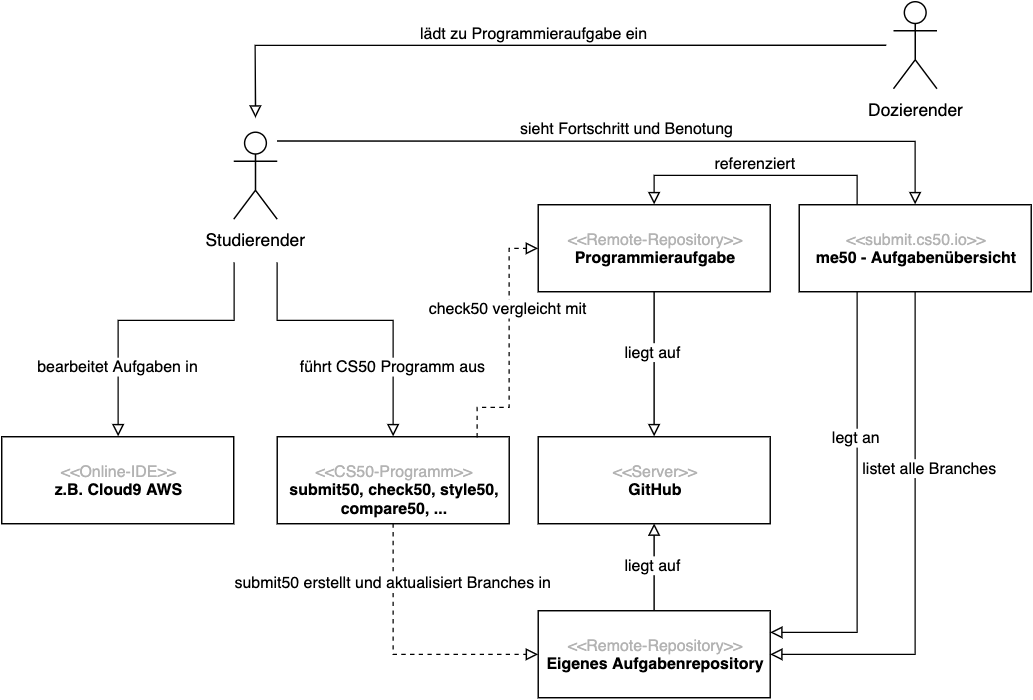
\includegraphics[width=\textwidth]{cs50-architektur}
    \caption{CS50 Architektur}
    \bildquelle{Eigene Darstellung}
    \label{fig:cs50-architektur}
\end{figure}

Teilnehmende dieses Online-Lehrangebots erhalten von den Dozierenden einen
Einladungslink zum Kurs. Dieser Link führt sie zur me50-Plattform
(https://submit.cs50.io/), welche gleichzeitig als Aufgabenübersicht dient. Die
Authentifizierung mit der Plattform geschieht dabei über GitHub. Auf dieser
Plattform können Studierende sowohl ihre Abgaben, als auch ihre Kurse
übersichtlich verwalten. Neben der Weiterleitung zur me50-Plattform wird
gleichzeitig in der me50-GitHub-Organisation ein leeres Repository mit dem
GitHub-Username des Teilnehmers angelegt.

Nach Annahme des Einladungslinks können Studierende in jeder beliebigen
Entwicklungsumgebung die Aufgaben auf der CS50-Plattform
(https://cs50.harvard.edu/) lösen. Das Korrigieren und Abgeben der Aufgabe
benötigt mindestens Zugriff auf die Kommandozeilen-Tools check50 und submit50.
Diese sind über den Python-Paketmanager frei verfügbar. Harvard stellt außerdem
eine kostenlose Online-IDE bereit, welche die genannten Python-Programme bereits
vorinstalliert zur Verfügung stellt.

Sobald der Studierende eine Aufgabe erfolgreich gelöst hat, kann er mithilfe des
Namens der Aufgabe die Lösung überprüfen und schließlich abgeben. Eine Abgabe
über die Konsole kann dann beispielsweise so aussehen:

\begin{lstlisting}[style=Bash]
    ~/hello/ $ submit50 cs50/problems/2021/x/hello
    Connecting......
    Authenticating...
    Verifying.........
    Preparing..................
    Files that will be submitted:
    ./hello.c
    Keeping in mind the course's policy on academic honesty, are you sure you want to submit these files (yes/no)? yes
    Uploading....
    .......
    Go to https://submit.cs50.io/users/ndhbr/cs50/problems/2021/x/hello to see your results.
\end{lstlisting}

Der Parameter \texttt{cs50/problems/2021/x/hello} im Aufruf von submit50 ist
der im vorherigen Abschnitt erläuterte Slug. Das Programm check50 wird ebenfalls
mit dem Slug als Parameter aufgerufen. Durch diese Information wissen die
Programme, mit welcher Aufgabe sie die Lösung des Teilnehmenden vergleichen
sollen.

Die letzte Zeile verlinkt erneut auf die me50-Plattform und zeigt dem
Kursteilnehmenden seine Abgaben dieser Aufgabe und seine damit erreichte
Punktezahl. Gleichzeitig verlinkt die me50-Plattform auf das vorher erstellte
GitHub-Repository des Lernenden. Die Plattform legt bei jeder neu abgegebenen
Aufgabe einen neuen Git-Branch für diese an. Nach der Abgabe des vorherigen
Beispiels hätte die Plattform folgenden Branch in dem Repository angelegt
\texttt{cs50/problems/2021/x/hello}. Durch die Commit-History in diesem Branch 
kann man später den Verlauf der Versuche nachverfolgen.

\paragraph{Probleme beim Einsatz an der OTH}
Die Toolchain von CS50 wäre grundsätzlich adäquat für den Einsatz an der
OTH-Regensburg. Jedoch ist eines der Projekte aktuell noch nicht Open-Source:
die Website zur Erstellung von neuen Kursen, Abgaben und Mitgliederverwaltung. 
Das heißt, dass der Quellcode dieses Projekts nicht öffentlich zugänglich ist.

Dieses Projekt ist gleichzeitig der größte Bestandteil des Netzwerks und ist
deshalb essenziell für die Verwendung der Werkzeuge an der Regensburger
Hochschule. Nach Rücksprache mit Herrn Carter Zenke der Harvard University ist
ein Neuaufbau dieser Website mit einhergehender Veröffentlichung als
Open-Source-Projekt gerade in Planung (siehe Anhang
\ref{appendix:carter-zenke}). Einen genauen öffentlichen Zeitplan hierfür gibt
es aktuell nicht. Infolgedessen ist ein Einsatz des CS50-Systems an der OTH zum
heutigen Datum nicht möglich.

\newpage
\subsubsection{Code FREAK der Fachhochschule Kiel}\label{code-freak}
\paragraph{Allgemeines}
Code FREAK ist eine All-in-one-Lösung für Online-Programmieraufgaben mit
automatisiertem Feedback. Die von der Hochschule Kiel entwickelte
Open-Source-Software soll den Einstieg in eine digitale Lernumgebung
vereinfachen. Die Zielgruppe von Code FREAK bezieht sich hierbei explizit auf
Hochschulen und Universitäten. \parencite{codefreak-startseite}

Des Weiteren wirbt Code FREAK mit einer \emph{LMS-Integration}. LMS ist die
englische Abkürzung für Learning Management System (Lernplattform). Viele
Schulen und Universitäten verwenden bekannte LMS-Systeme, wie Moodle, um Kurse,
Fächer und Studierende zu verwalten \parencite{moodle}. Dies hat den Vorteil,
dass Studierende kein extra Nutzerkonto für Code FREAK anlegen müssen. Sie
können sich direkt mit ihrem gewohnten Hochschulzugang anmelden.

\paragraph{Ablauf für Studierende}
Studierende können nach Anmeldung am System, an für sie sichtbaren Kursen
(Assignments) teilnehmen. Dies geschieht meist durch einen vom Dozierenden
generierten Einladungslink. Jedes Assignment enthält eine oder mehrere Aufgaben
(Tasks). Sobald der Einladungslink zum Assignment akzeptiert wurde, hat die
teilnehmende Person Zugang zu allen in dem Assignment enthaltenen Tasks. Die
einzelnen Aufgaben werden dann entweder über die integrierte
Online-Entwicklungsumgebung, durch Hochladen der Lösung, oder durch die Angabe
eines Git-Remote-Repository-Links bearbeitet.

Mit dem Klick auf die \glqq Start Evaluation\grqq{} Schaltfläche wird die
hochgeladene Lösung der Aufgabe überprüft. Die Ergebnisse der einzelnen
Test-Schritte werden in einem weiteren Tab visualisiert. Zusätzlich zu den
üblichen Unit-Tests enthalten die Test-Schritte unter Umständen auch
sogenannte \emph{Stylechecks}. Ein Stylecheck überprüft, ob der geschriebene
Code nach den für die Programmiersprache üblichen Konventionen formatiert ist.
Die Evaluation einer Aufgabe kann beliebig oft wiederholt werden. Wenn alle
Tests der Aufgabe bestanden wurden, wird der Task mit einem grünen Haken
versehen. So sieht der Schüler in der Assignment-Ansicht auf einen Blick, welche
Aufgaben er bereits gelöst hat und an welchen Aufgaben er noch arbeiten muss.

\paragraph{Ablauf für Lehrende}
Lehrende erstellen in Code FREAK Aufgaben in einem sogenannten \emph{Task Pool}.
In diesem Task Pool können beliebig viele Tasks angelegt werden. Zusätzlich zum
Verfassen einer ausführlichen Anleitung, enthält Code FREAK bei der Erstellung
neuer Tasks außerdem einen Bereich, um einzelne Test-Schritte festzulegen. Diese
Schritte erlauben es neben den vorher erklärten Unit-Tests (siehe
\autoref{unit-tests}) zusätzliche Tests, wie beispielsweise Stylechecks,
nacheinander auszuführen.

Anschließend erstellen Lehrende Assignments, welche aus den vorher angelegten
Tasks im Task Pool bestehen. Der Task Pool hat den Vorteil, dass mehrere Kurse
dieselben Aufgaben wiederverwenden können, ohne diese redundant anlegen zu
müssen. Dieses Vorgehen erhöht die Wartbarkeit der Aufgaben ungemein. Die
Einzelansicht eines Kurses erlaubt es zusätzlich eine optionale Deadline sowie
eine maximale Bearbeitungsdauer anzugeben. Außerdem gibt es eine Schaltfläche,
um Ergebnisse und Bewertungen der Studierenden als .CSV-Datei zu exportieren.
Die Lösungsversuche der Teilnehmenden werden wiederum als .ZIP- oder als
.TAR-Datei zum Herunterladen angeboten.

\paragraph{Architektur}
Code FREAK wird als fertiger Docker-Container ausgeliefert. Docker ist eine
Software, um mithilfe von Containervirtualisierung einzelne Anwendungen
voneinander zu isolieren. Durch die Containervirtualisierung werden unter
anderem viele Abhängigkeits-, Sicherheits-, Netzwerk- und Einrichtungsprobleme
beseitigt. Der Container enthält alle Bibliotheken und Abhängigkeiten, die die
Software für die Laufzeit benötigt \parencite{docker}. Docker entstand auf Basis
von Linux-Containern, welche einen oder mehrere Prozesse vom restlichen System
isolieren können 
\parencite{linux-container}.

Durch diese Handhabung kann Code FREAK mit nur einem Befehl in der
Kommandozeile installiert und gestartet werden. Die Software benötigt
grundsätzlich nur einen Container. Benutzt ein Studierender jedoch die
integrierte Online-Entwicklungsumgebung, muss für jede Instanz ein zusätzlicher
Container mit der Laufzeitumgebung der IDE gestartet werden. Jeder weitere
Container benötigt weiteren Arbeitsspeicher und erhöht die Prozessorlast.

\paragraph{Probleme beim Einsatz an der OTH}
Beim Einsatz von Code FREAK an der Hochschule Regensburg gibt es einige
Probleme. Das erste Hindernis bezieht sich auf den vorher erwähnten
Arbeitsspeicher. Die Praxis zeigt, dass eine Instanz der Online-IDE schon nach
wenigen Quellcodedateien rund drei Gigabyte an Arbeitsspeicher verwendet. Um
eine reibungslose und parallele Nutzung für alle Studierenden des Kurses
gewährleisten zu können, werden dementsprechend sehr hohe Serverkosten fällig. 
\parencite{codefreak-memory-problem}

Eine weitere Hürde ist die Stabilität der Software. Code FREAK befindet sich,
Stand \today, mitten in der Entwicklung, weshalb einige Funktionen und Features
noch nicht ordnungsgemäß funktionieren -- darunter die vorher angeworbene
LMS-Integration \parencite{codefreak-docs}. Zum heutigen Zeitpunkt ist das
\ac{ldap} die einzige Möglichkeit, sich mit dem System zu authentifizieren. Ein
eigenes Anmeldeverfahren gibt es bisher noch nicht.

LDAP steht für Lightweight Directory Access Protocol und ist ein
Netzwerkprotokoll zur Durchführung von Abfragen und Änderungen in einem 
verteilten Verzeichnisdienst. LDAP ist der de facto Industriestandard für
Authentifizierung und Autorisierung. \parencite{ldap}

Der Kurs Digital Skills soll den Teilnehmenden einen Überblick über den
Arbeitsalltag eines Informatikers geben. Dazu gehört unter anderem die
Kommandozeile. Eine Anforderung der Lernplattform ist deshalb, dass man
optional neue Aufgaben herunterladen und Lösungsversuche über Befehle in der
Kommandozeile testen und abgeben kann. In Code FREAK kann man Aufgaben lediglich
über die Oberfläche testen und abgeben.

\newpage
\subsubsection{GitHub Classroom}
\paragraph{Allgemeines}
GitHub Classroom ist ein weiterer Kandidat für den Einsatz an der
Hochschule Regensburg. Die Plattform ermöglicht die automatisierte
Erstellung von Repositorys auf GitHub. Außerdem hilft Classroom dabei,
Aufgabenvorlagen und dazugehörige Abgaben einfach zu verwalten und automatisch
zu benoten. Dabei enthalten die von GitHub Classroom erstellten
Aufgaben-Repositorys bereits vorkonfigurierte Zugriffskontrollen.
\parencite{github-classroom-startseite}

\paragraph{Ablauf für Studierende}
Studierende bekommen pro Programmieraufgabe einen Einladungslink. Nach Annahme
der Einladung wird für jeden Studierenden automatisch ein Repository für die
jeweilige Aufgabe angelegt. Dieses Repository enthält die Vorlage, welche zum
Bearbeiten der Aufgabe benötigt wird.

Sobald der Studierende eine Lösung zur Korrektur abgeben möchte, kann er per
Push die Änderungen in das Remote-Repository hochladen. Je nach Konfiguration
der Aufgabe starten daraufhin serverseitig ein oder mehrere Tests. Wenn alle
Tests bestanden sind, hat der Studierende die Aufgabe erfolgreich abgeschlossen.

\paragraph{Ablauf für Lehrende}
Um eine Aufgabe in GitHub Classroom zur Verfügung zu stellen, bedarf es zuerst
einer GitHub Organisation, sowie eines Kurses in GitHub Classroom. Sobald beides
erstellt ist, können Lehrende neue Assignments (Aufgaben) mithilfe von
bestehenden Vorlage-Repositorys erstellen. In der Vorlage befindet sich in der
Regel ein Ordner mit Tests, welche das Ergebnis des Programms prüfen sollen.
In GitHub Classroom kann demnach eine Reihe an Kommandozeilenbefehlen festgelegt
werden, die dann diese Tests ausführen und je nach Ergebnis bepunkten.

Eine Übersicht über die Abgaben und erreichten Punktzahlen der Studierenden kann
sich der Dozierende jederzeit per Klick auf eine Aufgabe anzeigen lassen.
Gleichzeitig ist es in dieser Ansicht möglich, alle Noten als .CSV-Datei und
alle Repositorys als .ZIP-Datei herunterzuladen.

\paragraph{Architektur}
GitHub Classroom ist ein Bildungsservice der Firma GitHub Inc. und ist, Stand
\today, kostenfrei \parencite{github-classroom-kostenlos}. Die Software basiert
auf der Automatisierung von Repositorys. Jeder bei GitHub registrierte Nutzer
kann einen sogenannten \emph{Classroom} erstellen und darin Aufgaben auf
Basis vorhandener öffentlichen GitHub-Repositorys erstellen.

\paragraph{Probleme beim Einsatz an der OTH}
Es gibt keine Möglichkeit, das System von GitHub Classroom auf einem lokalen
Git-Server zu replizieren. Aufgrund dessen schafft man sich durch die
Verwendung von Classroom eine externe Abhängigkeit an GitHub. Dies kann unter
Umständen zu erheblichen Problemen führen, wenn der Dienst beispielsweise
nicht erreichbar oder eingestellt wird. Durch die Größe und Infrastruktur des
Unternehmens ist jedoch weder ein häufiger Ausfall noch eine Auflösung des
Dienstes zu erwarten.

Eine weitere Herausforderung ist der Bedarf an weiterer Software. GitHub
Classroom alleine ist nicht ausreichend, um als vollständige Lernplattform für
den Kurs Digital Skills zu fungieren. Hier bietet es sich an, eine eigene
statische Website mit Anleitungen und Erklärungen zu bauen, welche dann jeweils
auf Classroom Einladungslinks verweist. Als Online-Entwicklungsumgebung kann der
Dienst Replit verwendet werden. In Replit ist es möglich, ein vorhandenes
Git-Repository als Template (Vorlage) für eine neue Umgebung zu verwenden.
Dieses Template könnte dann Hilfsprogramme für den Git-Workflow enthalten. Der
Vorteil daran: Studierende bekommen erste Erfahrungen mit der Kommandozeile,
müssen jedoch keine komplexen Git-Kommandos im Zusammenhang mit GitHub Classroom
absetzen.

\subsubsection{Bewertung und Entscheidung der vorhandenen Systeme}
Die auf der nächsten Seite folgende \autoref{fig:systemvergleich} visualisiert
die erläuterten Systeme und bewertet diese anhand der vorher definierten
Anforderungen (siehe \autoref{anforderungsanalyse}). Die blau hinterlegten
Zeilen repräsentieren die nichtfunktionalen Anforderungen. Alle rosa
hinterlegten Zeilen wiederum repräsentieren die funktionalen Anforderungen aus
der Sicht des Teilnehmers. Der letzte, gelb hinterlegte, Teil spiegelt
schließlich die funktionalen Anforderungen aus der Sicht der Lehrenden wider.

Die erste Spalte enthält die Namen der Anforderungen, während in der zweiten
Spalte die Gewichtungen der Anforderungen aufgeführt sind. Der valide Bereich
dieser Spalte befindet sich zwischen einschließlich 0,00 und 1,00. Eine 1,00
bedeutet, dass die Anforderung für den Einsatz an der Hochschule sehr wichtig
ist. Je niedriger der Wert, desto unwichtiger die Anforderung.

Die Spalten drei, vier und fünf enthalten die Bewertungen, in welchem Grad die
Systeme die Anforderungen erfüllen. Hierbei gilt ähnlich wie bei der Gewichtung:
je höher der Wert, desto besser. Der valide Bereich befindet sich hier jedoch
zwischen 0,0 und 3,0. Der Wert 0 bedeutet, dass das Feature nicht vorhanden ist,
oder nicht zutrifft. Eine 3 wiederum stellt eine völlige Übereinstimmung mit der
geforderten Anforderung dar. Alle Werte dazwischen bilden lineare Zwischenwerte.
Die Spalten enthalten hierbei das Ergebnis der Multiplikation aus der Bepunktung
mit der Gewichtung. Sowohl die Punkteverteilung und Festlegung der Gewichtungen
als auch die Recherchen über die gegebenen Plattformen und Anforderungen wurden
von Andreas Huber durchgeführt.

\begin{figure}[H]
    \centering
    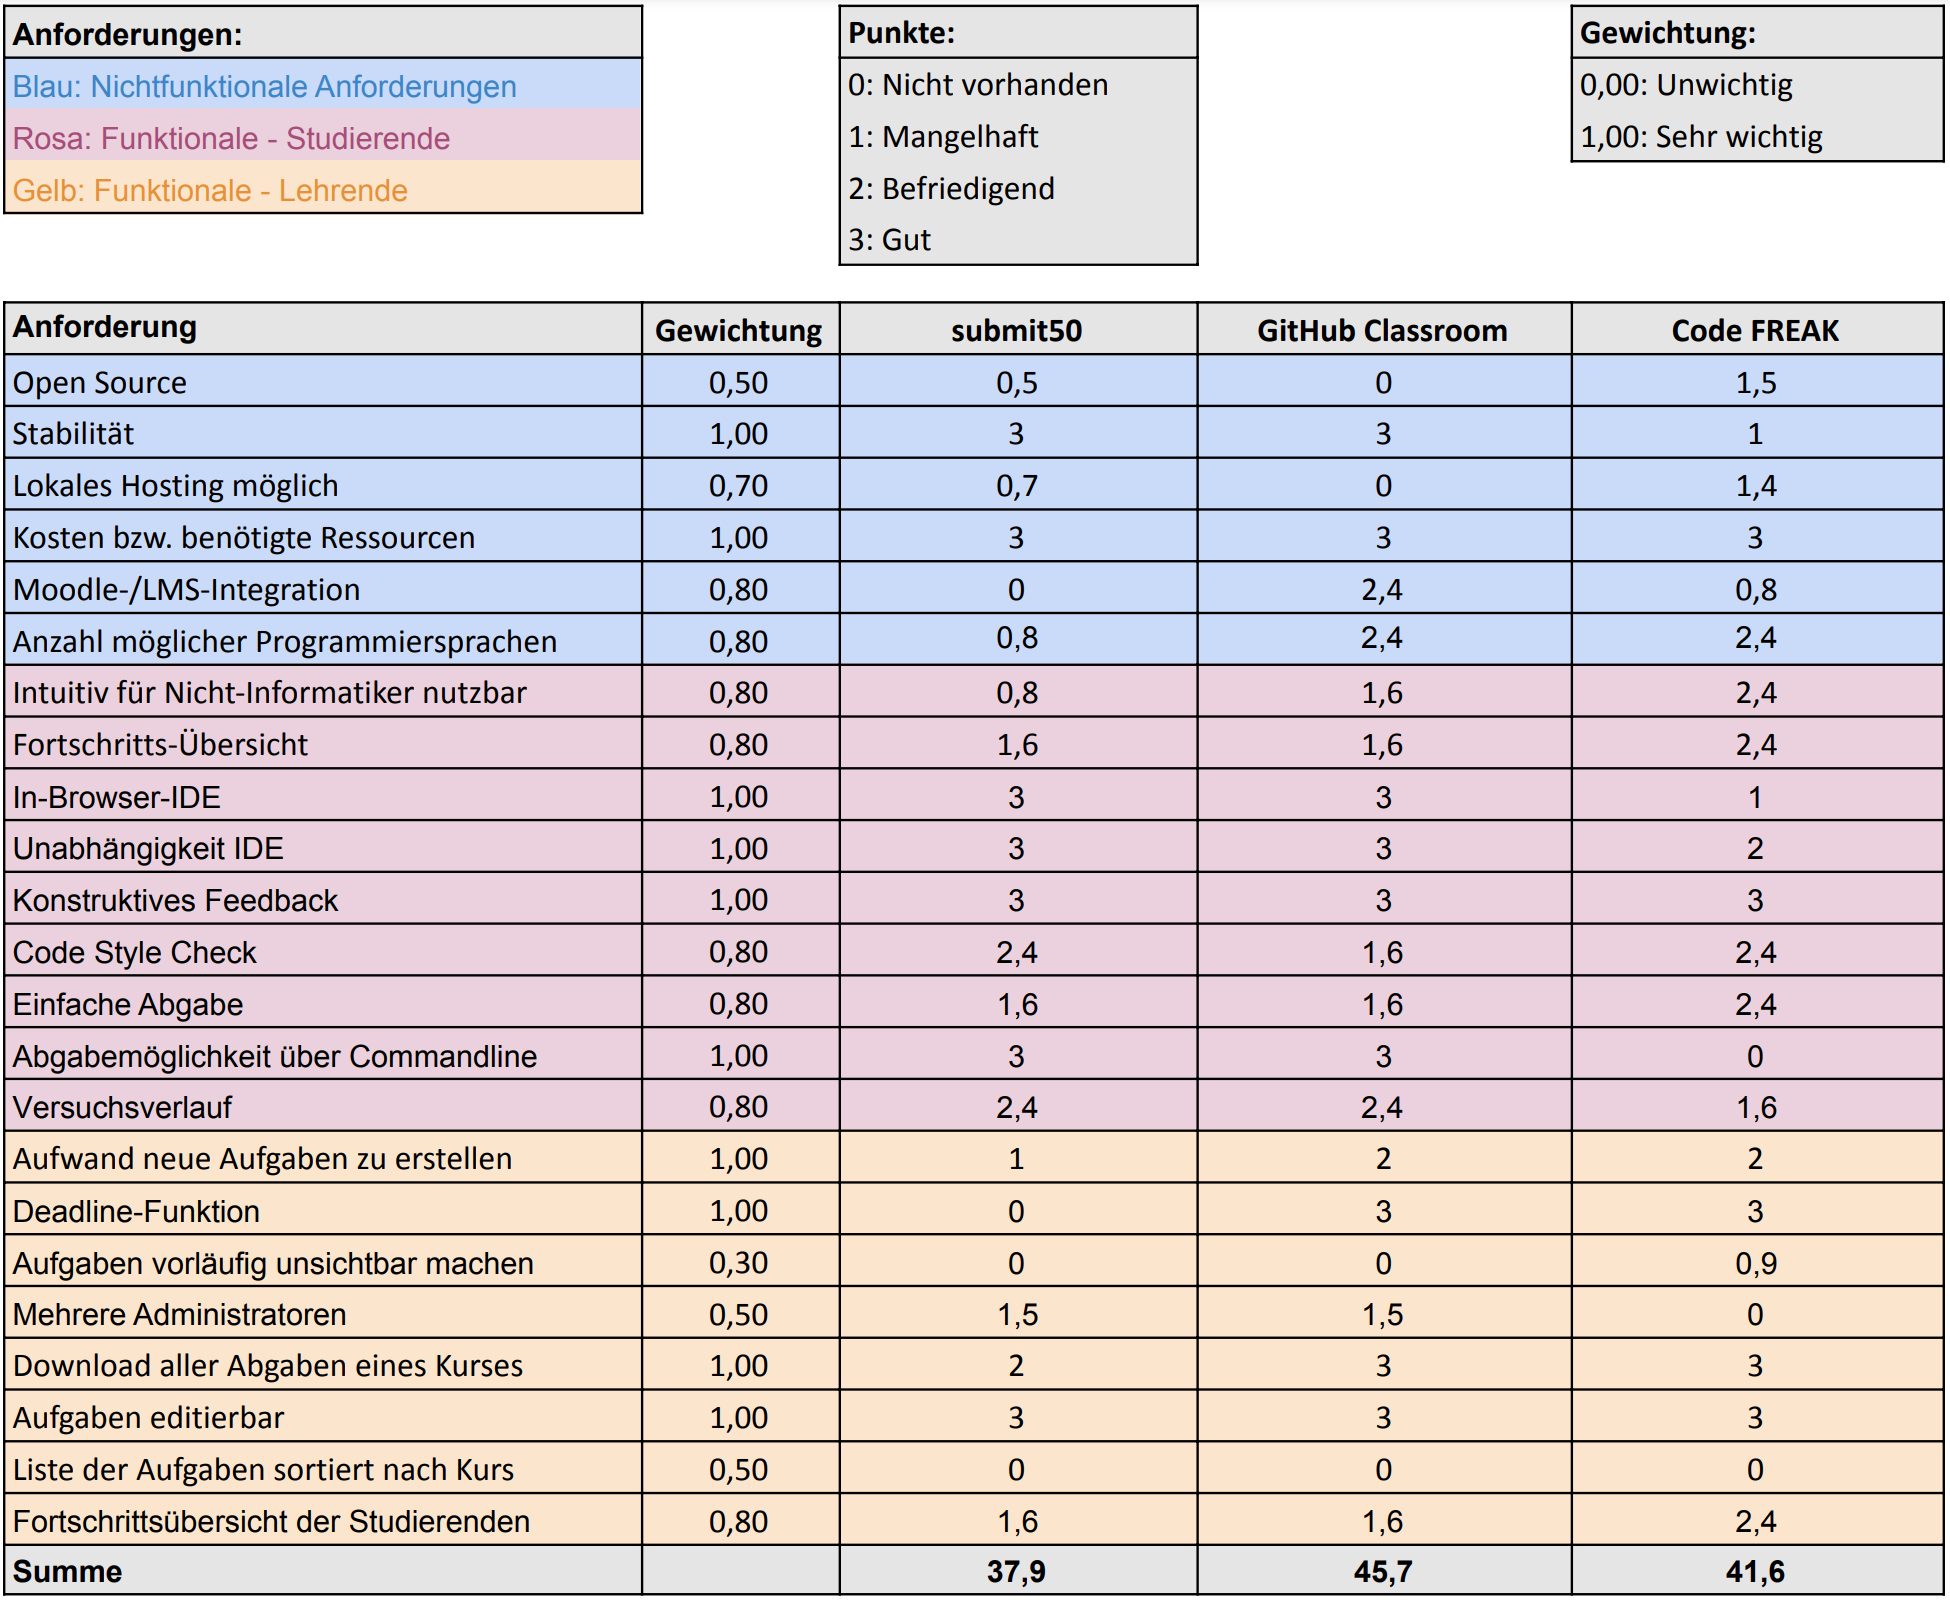
\includegraphics[width=\textwidth]{systemvergleich}
    \caption{Vergleich und Benotung der Systeme}
    \bildquelle{Eigene Darstellung}
    \label{fig:systemvergleich}
\end{figure}

\newpage

Zusammenfassend befinden sich in der letzten Zeile die Summen der Benotungen. In
diesem Fall hat das System mit GitHub Classroom die meisten Punkte erreicht und
wird somit als geeigneter Kandidat für die Programmierplattform des
Zusatzstudiums Digital Skills weiter evaluiert.